\documentclass[14pt,utf8,hyperref={pdfpagelabels=false}]{beamer}
\usepackage{etex}
\usepackage{media9}

\usepackage[utf8]{inputenc} % hyperref broken with utf8x
\usepackage[C40,T1]{fontenc}

\usepackage{graphicx}
\usepackage{array}
\usepackage{multirow}

\usetheme{moulardthesis}

\DeclareUnicodeCharacter{00A0}{~}

\title{Toward Debian-powered robots?}

\author[T\.~Moulard]{Thomas~Moulard}


\date{June 2013}

\begin{document}

{
  \usebackgroundtemplate{%
    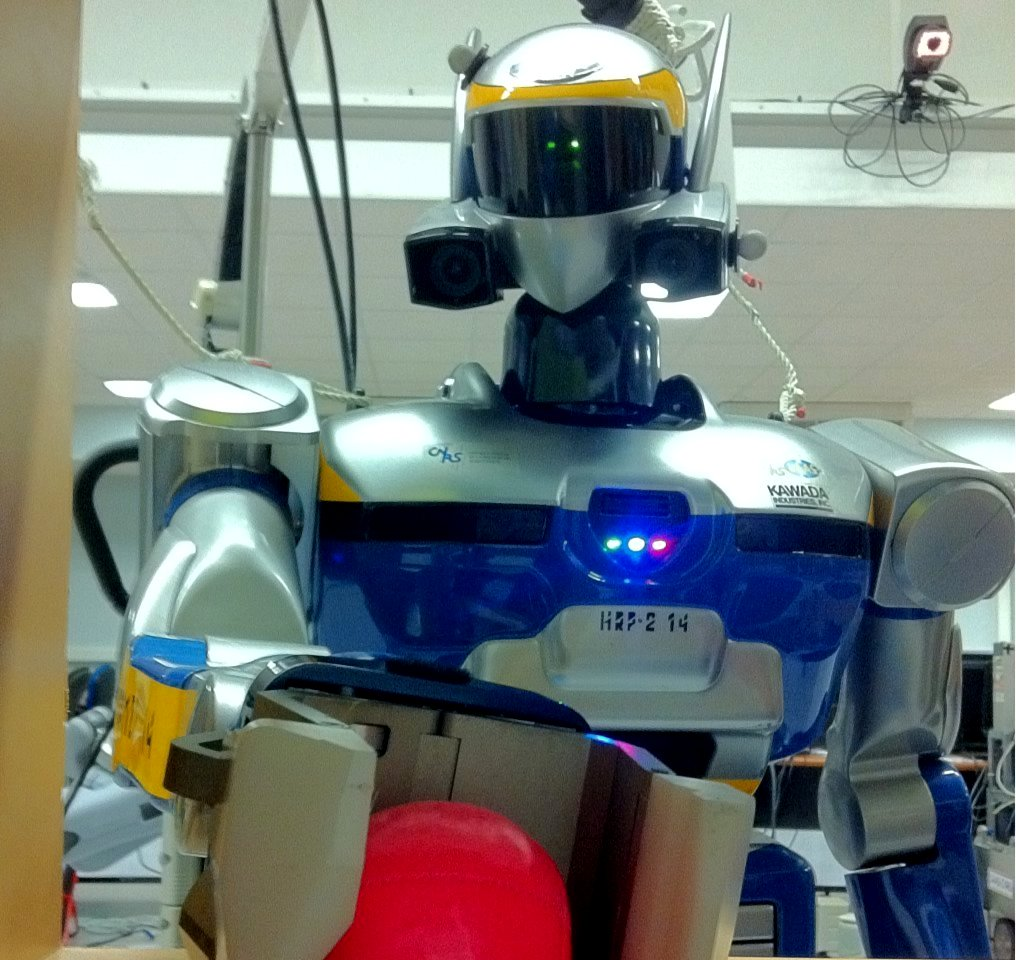
\includegraphics[width=\paperwidth,height=\paperheight]{%
      images/demo1.jpg}}
  \begin{frame}[plain]
    \titlepage
  \end{frame}
}

\begin{slideDecision}
  \frametitle{Robots are everywhere!}

  % FIXME: add cool robots images.
\end{slideDecision}


\begin{slideDecision}
  \frametitle{What software need robots?}

  \begin{description}
    \item[Middlewares] OpenRTM, ROS.
    \item[Simulators and development framework] Choreonoid, Gazebo,
      Morse, OpenHRP, OpenRAVE.
    \item[Development libraries] OpenCV, PCL (Point Cloud Library), ViSP.
  \end{description}

  Most of them lack Debian packaging.

\end{slideDecision}

% FIXME: add various screenshots of software.

\begin{slideDecision}
  \frametitle{Why does it matter?}

  \begin{itemize}
    \item Robotics is promising.
    \item Most of the best tools are open-source.
    \item Robots may become day-to-day home/office appliance at some
      point. Or already are: Roomba!
    \item This is the time. The moment when ``research projects'' will
      become industrial platforms is \emph{now}.
  \end{itemize}

\end{slideDecision}

\begin{slideDecision}
  \frametitle{How can you help?}

  \begin{itemize}
    \item Not all roboticists are open-source experts.
    \item Students and researchers need a working environment.
    \item Debian can \emph{provide this}.
  \end{itemize}

  \vspace{1cm}

  You can help by: packaging robotics software and reporting
  bugs on existing software.

\end{slideDecision}

\maxFrameImage{images/hrp2-thx.jpg}

\end{document}
